\chapter{Testing}

\section{Experimental design}
The tests are run by reading a dataset into a dynamic array, which is populated
outside the timer loops. The threads are then created with a reference to the
trie and the array, which has a built in iterator. 
The dynamic array is a threadsafe multiple-readers structure to
allow the threads to concurrently extract words from the dataset after first
reading them into memory. Not only must the accesses be thread-safe, but
a shared thread-safe iterator is needed.

We have therefore implemented a simple CREW (concurrent read exclusive write)
vector for this purpose. The base footprint of this is a memory consumption
of 8 times the word count bytes from pointers, plus the size of the dataset
itself. It works by doing an atomic {\keyword AO\_fetch\_and\_add}, and
exploits the indexing of the array.

The structure is compared with the \STL map implementation for a baseline result.
The tests are designed to test the structure under both uniform distribution and
under real-world dictionary use. In order to show that it is possible to obtain
better results than sequential insertion, the number of threads is varied
across the tests and trie variants.

More complex trie implementations are not tested, as the source code has not
been made available in any of the referenced material.

Using the Gnu Scientific Library taus random number generator and a predefined
seed, 30 million random strings were generated. This method was chosen to
obtain a uniformly distributed data on a larger scale, which is chosen to
obtain the shallowest trie possible given the number of elements.

%GSL\_RNG\_SEED=110604190045 GSL\_RNG\_TYPE=taus /usr/bin/time -v ./tests/bin/seq/seq\_map > map\_30M.log 2>&1 
\begin{table}[h!]
    \centering
    \begin{tabular}[here]{l l l l l l}
        \hline
        Dataset    & Distinct   & Strings      & Avg     & Size (MB)& Size (MB)\\
                   &            &              & length  & distinct & total    \\\hline
        30M Random & 29,990,518 & 30,000,000   & 9.00    & 228.84   & 270.00\\
        Shakespeare&  31,229    & 340,039      & 5.56    & 0.21     & 18.91\\
        Newsgroups & 463,269    & 6,046,538    & 7.63    & 8.59     & 46.13\\
        \hline
    \end{tabular}
    \caption{Characteristics of the datasets used for insertions and self-search.}
    \label{tab:datasets}
\end{table}

The tests will be run on three different setups, to determine the impact of
increased hardware parallelism, by utilizing 2, 4 and 8 cores respectively.

\begin{table}[h!]
    \centering
    \begin{tabular}[here]{ l l l l }
        \hline
                  & Intel \\\cline{2-4}
                  & Core 2 Duo T9300 & Core i7-950  & Xeon E5420 \\ \hline
        Abbrevation & C2D & i7 & Xeon \\ 
        CPU speed   & 2.50 GHz & 3.06 GHz & 2.50 GHz \\
        No. CPUs    & 1 & 1 & 2 \\
        Phys. Cores & 2 & 4 & 8 \\
        Virt. Cores & 0 & 4 & 0 \\
        L1/L2/L3 size(kB) & 64/6.144 & 128/1024/8.192 & 128/12.288\\
        L1/L2 cacheline(B) & 64/64 & 64/64 & 64/64\\
        %TLB entries & \\
        Memory (MB) & 4,096 & 8,192 & 32,768 \\
        Memory type & DDR2 800 & DDR3 1333 & DDR2 800 \\a
        Memory channels & 2 & 3 & 2 \\
        %Memory latency  & 
        Linux Kernel    & 2.6.38 & 2.6.38 & 2.6.36 \\
        Processor type  & 64-bit & 64-bit & 64-bit \\\hline
    \end{tabular}
    \caption{Characteristics of the used testing machines.}
    \label{tab:cpucpecs}
\end{table}

The Core 2 Duo machine is a Dell Laptop, chosen for its dual-core CPU.
The Xeon machine is a server workstation at DIKU, with two Xeon E5420 CPUs,
but is shared with many other students, which means that the workload
under testing was not under our control. The i7 machine was used for its
quad-core CPU, and with hyperthreading showing up as an octo-core, where four
of them are virtual, provides an interesting comparison with the Xeon machine,
which has 8 physical cores. The i7 machine was used for primary testing.

The tests themselves are run by running 10 iterations of the dataset. The order
of the elements is randomized before inserting, and again before searching, to
avoid searching in the same order they were inserted.


\subsection{Datasets}
The different datasets result in different node and bucket counts for each
bucket size. These counts give an indication of the structure of the trie,
and are needed to understand the results, when changing the sizes.

\begin{table}[h]
    \centering
    \begin{tabular}[here]{ l l l l }
        \hline
        Bucketsize& Node count  & Bucket count & Average load  \\\hline
        32        &  254,080    & 13,408,608   & 2.23\\
        64        &  254,080    & 13,408,608   & 2.23\\
        128       &  58,396     & 3,225,230    & 9.29\\
        256       &  4033       & 250,047      & 119.94\\
        \vdots    &  \vdots     & \vdots       &\\
        4096      &  4033       & 250,047      & 119.94\\\hline 
    \end{tabular}
    \caption{Bucket and node counts for the various bucket sizes using the
        30M dataset. Average load indicates the average number of elements
        per bucket on termination.}
    \label{tab:bncounts_30M}
\end{table}

With the counts being the same for several of the sizes, any difference in performance
during insertion must be caused by bursting. When the containers are allowed to grow,
the upper bound on insertion and bursting becomes more important.

The shakespeare dataset is chosen for its real-world character distribution, and will
therefore present a good test-case for dictionary use of the structure.

\begin{table}[h]
    \centering
    \begin{tabular}[here]{ l l l l }
        \hline
        Bucketsize&  Node count & Bucket count& Average load  \\\hline
        32        &  4,511      & 12,396      & 2.52 \\
        64        &  2,565      & 9,155       & 3.41 \\
        128       &  1,372      & 6,432       & 4.85 \\
        256       &  659        & 4,203       & 7.43 \\
        512       &  340        & 2,770       & 11.27\\
        1024      &  155        & 1,750       & 17.85\\ 
        2048      &  99         & 1,231       & 25.37\\ 
        4096      &  44         & 580         & 53.84\\\hline 
    \end{tabular}
    \caption{Bucket and node counts for the various bucket sizes using the Shakespeare
        dataset.}
    \label{tab:bncounts_shakespeare}
\end{table}


By using a dataset that is perhaps more real world applicable, the structure is
evaluated as a means of storing data for web scraping and analysis. The dataset has a 
larger alphabet than the others, resulting in the requirement to increase
node size to 256 from 128.

\begin{table}[h]
    \centering
    \begin{tabular}[here]{ l l l l }
        \hline
        Bucketsize& Node count  & Bucket count & Average load  \\\hline
        32        &  61,502     & 176,065      & 2.63\\
        64        &  34,297     & 140,498      & 3.30\\
        128       &  19,594     & 108,208      & 4.28\\
        256       &  11,538     & 79,400       & 5.83\\
        512       &  6,665      & 55,016       & 8.42\\
        1024      &  3,663      & 36,726       & 12.61\\ 
        2048      &  1,888      & 24,122       & 19.21\\ 
        4096      &  911        & 15,710       & 29.49\\\hline 
    \end{tabular}
    \caption{Bucket and node counts for the various bucket sizes using the
    newsgroups dataset. Average load indicates the average number of elements
    per bucket on termination.}
    \label{tab:bncounts_ngrp}
\end{table}

With the dictionary sets having larger skew, the structure is more sensitive to
the bucket sizes (table \ref{tab:bncounts_shakespeare} and
\ref{tab:bncounts_ngrp}). As such, a more continuous scaling is expected for
these sets.

\section{Sequential results}
For assessing the relative performances under a sequential environment, first a
baseline measurement of the {\keyword STL::Map} structure is made, on each of
the test machines.

Basic MAP result using the 30M dataset.
\begin{table}[h!]
    \centering
    \begin{tabular}[here]{ l l l }
        \hline
        Machine   & Insertion time & Self-search time  \\\hline
        C2D       & NA             & NA                \\\hline
        i7        & 112.74         & 110.45            \\\hline
        Xeon      & 231.33         & 231.56            \\\hline 
    \end{tabular}
    \caption{Base results for the STL::Map container, using the 30M random strings set.}
    \label{tab:maptimes}
\end{table}

Here, the primary difference of the machines lies in the amount of memory
available. Since the structure uses more than 4500 MB with the chosen dataset,
the Core2Duo setup uses paging to obtain the needed memory, and as such incurs
a huge performance hit when compared to the other two.

To verify this, Valgrind was run with the Massif heap profiler, showing an
allocation size of 434MB. Assuming linear scaling, this is slightly lower than
the observed 4450MB. Massif and valgrind was unable to run on the full 30M set,
because of added memory overhead.

The binary trees also take an impact on increased bucket sizes, which
is a increased emphasis on insertion order may create deep buckets, which also
shows slightly in the insertion phase (see Figure \ref{fig:seq_30m} on
Page \pageref{fig:seq_30m}).

The expected constant-time insertion into unsorted arrays is evident, showing
an insertion time of $24$ to $38$ seconds. This container then pays on search
by linear search times. The reverse cost is seen for sorted arrays as expected.

The {\keyword map} bucket scales second best on insertion with larger bucket
sizes, but shows a large jump in memory use when compared to the other buckets,
with smaller bucket sizes. This is mainly attributed to the {\keyword map}
using dynamic resizing, where the chosen size of 64 elements is just above a
reallocation limit.

\begin{landscape}
    \begin{figure*}[H]
        \subfloat[Insert]{
            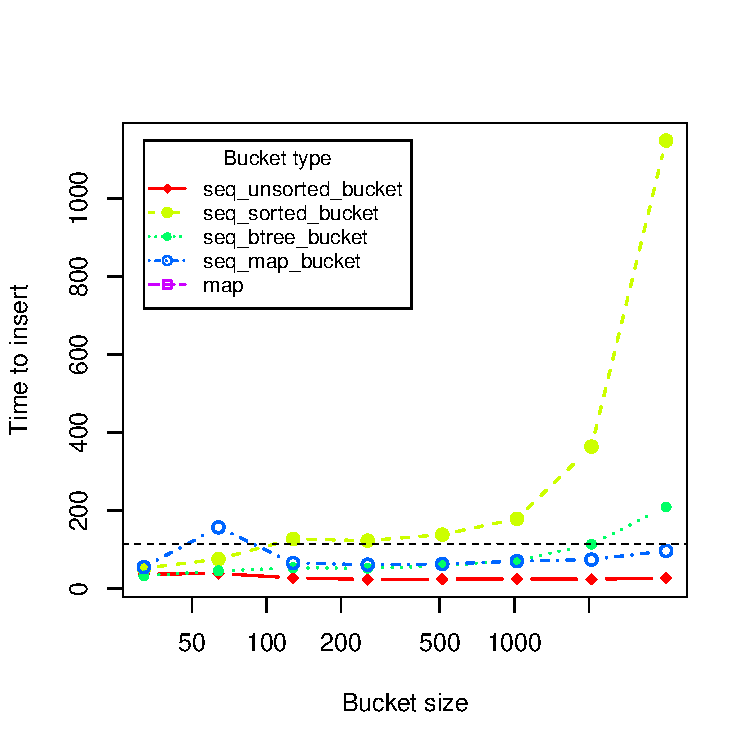
\includegraphics[width=1.0\textwidth]{plots/i7_30m_insert}
        }
        \subfloat[Search]{
            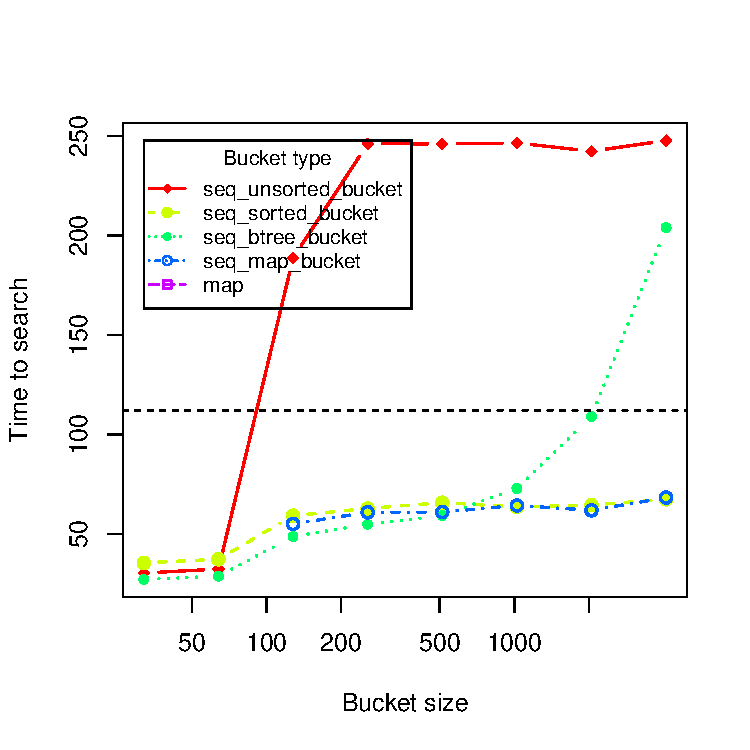
\includegraphics[width=1.0\textwidth]{plots/i7_30m_search}
        }
        \caption{Sequential test: Scaling of insertion and self-search times
        using the 30M Random dataset, with varying bucket sizes from 32 to
        4096. The {\keyword map} time is shown for reference as a dotted line.}
        \label{fig:seq_30m}
    \end{figure*}
\end{landscape}



\clearpage
\section{Parallel scaling}
In testing the parallel scaling of the different burst trie variants,
testing has been done on all three machines in order to evaluate scaling
to the number of CPUs.

The first improvement made was to the locking method of the nodes. Here in
Figure \ref{fig:globallock}, the difference is shown.
\begin{figure}[h!]
    \centering
    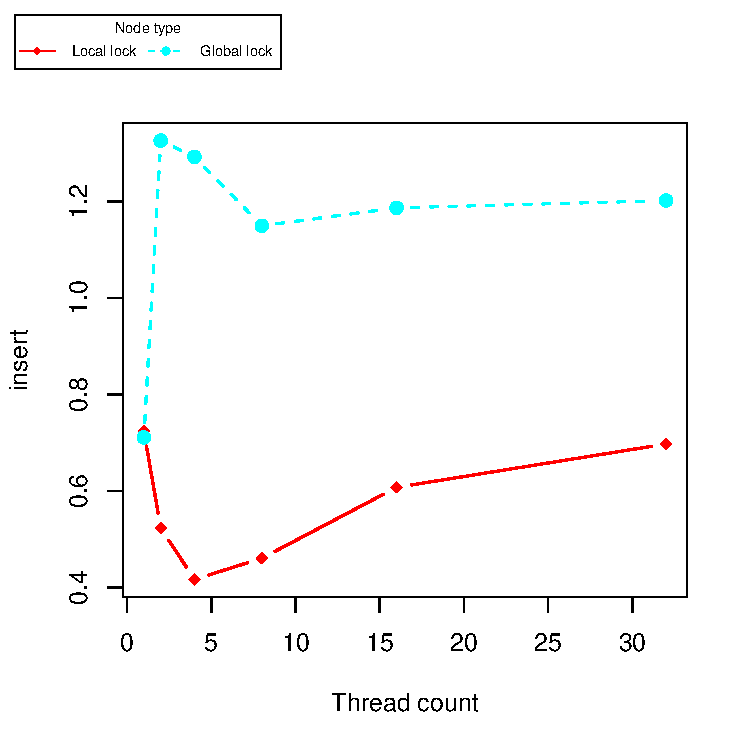
\includegraphics[width=0.5\textwidth]{plots/ts_locking}
    \fxwarning{Fix globallock plot}
    \caption{Thread scaling with global and local locking on the i7 machine (quad core),
    and the newsgroups dataset.}
    \label{fig:globallock}
\end{figure}
It is clear that the global lock is not a viable solution, these tests
show a clear bottleneck already beginning to show at 2 cores for insertions.
As such, insertions using more than a single thread are slower, since no
parallelism is gained, while synchronization of caches and locking is added.
The local locking on the other hand benefits from adding threads up to the
number of available CPUs.



While the sequential results show a clear tendency towards increased runtime
with larger containers, the sizes also influence the structure of the trie.
This means that different bucket sizes will scale differently.

\begin{table}[h]
    \centering
    \begin{tabular}[here]{ l l l l }
    \hline
        Bucket type            & Size & Insert & Search\\\hline
        %
        STL::Map               & 256  & 1.768  & 5.441\\
        Sorted dynamic array   & 256  & 3.301  & 5.261\\
        Unsorted dynamic array & 64   & 1.030  & 3.644\\
        Unsorted dynamic array & 128+ & ~0.600 & 6.108\\
        Binary tree            & 128  & 1.523  & 4.938\\
        Binary tree            & 32   & 0.979  & 5.680\\
    \hline
    \end{tabular}
    \caption{i7 30M: Best observed speedup factor for each bucket in the 30M
    dataset for up to 32 threads on the i7 quad-core machine (virtual
    octo-core). Results shown as best insertion time and best search time. The
    same size performed best on both if there is only one line.}
    \label{tab:speedups_30m_i7}
\end{table}
\begin{table}[h]
    \centering
    \begin{tabular}[here]{ l l l l }
    \hline
        Bucket type            & Size & Insert & Search\\\hline
        %
        STL::Map               & 128  & 1.054  & 2.120\\
        STL::Map               & 4096 & 0.702  & 2.564\\
        Sorted dynamic array   & 32   & 1.584  & 2.533\\
        Sorted dynamic array   & 4096 & 0.825  & 2.970\\
        Unsorted dynamic array & 64   & 1.065  & 2.177\\
        Unsorted dynamic array & 4096 & 0.603  & 3.941\\
        Binary tree            & 1024 & 1.714  & 2.218\\
        Binary tree            & 4096 & 1.293  & 2.530\\
    \hline
    \end{tabular}
    \caption{i7 Shakespeare: Best observed speedup factor for each bucket in
    the shakespeare dataset for up to 32 threads on the i7 quad-core machine
    (virtual octo-core). Results shown with best insertion time and best search
    time. The same size performed best on both if there is only one line.}
    \label{tab:speedups_shsp_i7}
\end{table}

The results from the 30M dataset (table \ref{tab:speedups_30m_i7} and page
\pageref{fig:ts_i7_30m}) show that it
is possible to obtain speedup factors of up to $6.1$ with a fully concurrent
locking mechanism on an octo-core system. With this as the reference, the gains of
a factor $3.3$ on insertions and a factor $5.2$ on searches for the sorted dynamic
arrays seem respectable. The sorted dynamic array with a size of 256 is the
only structure/size combination that scales well on both insertion and search. The
four virtual cores (Hyper-threading) have a greater impact on performance than
expected, with most tests scaling up to 8 threads. The scaling of the i7 is
high enough, that the results from the Xeon setup have been discarded due to
inconsistencies from uncontrolled load factors. The scaling of the two resp.
four cores can be seen in on page \pageref{fig:ts_shsp}.

The greatest gains appearing from unsorted array concurrency is evidence that
the locking favors heavy work in the leaves. This fits perfectly with the
expected node-level parallelism, which also explains why the greatest gains in
insertion is seen with sorted arrays, being the only bucket structure with
linear insertion times, and thereby up to $O(b^2)$ bursting times.

It is somewhat surprising that the searches take such a big hit from the
locking, seen in the larger unsorted array cases, and when comparing with
the shakespeare set (table \ref{tab:speedups_shsp_i7}). The shakespeare tests
result in a much smaller trie, and the continuous scaling of the trie (seen in
Table \ref{tab:bncount_shakespeare}) allows us to conclude that the overhead
from locks is dominant for smaller containers. This is seen by all containers
favoring larger buckets, meaning a shallower trie and less locks. The results
for the shakespeare and newsgroup sets show the same conclusion, the scaling
    can be seen on page \pageref{fig:ts_i7_nsgrp}.

The empirical concurrency of the read-locks is hereby reduced. The difference
is even greater on the Xeon machine, where the maximum speedup factor observed
for searching was $4.1$ for the 30M set. The Xeon results are very inconsistent
    due to shared resources with other students, and have been only used for
    reference.
